\chapter{Background}
% xzt: do not delete
\pagestyle{plain}

This is chapter 2.

\section{Figure}

Fig.~\ref{fig:navigation_examples} is an example from \cite{xie2024scope, xie2023drl, xie2023stochastic, xiao2022autonomous, chen2022semantic, xie2021towards} for placing a figure in the dissertation. For convenience, you can put the figures of one chapter in a single folder. 
  
\begin{figure}[t]
    \centering
    \subfigure[Simulated indoor environment]
    {
        \centering
        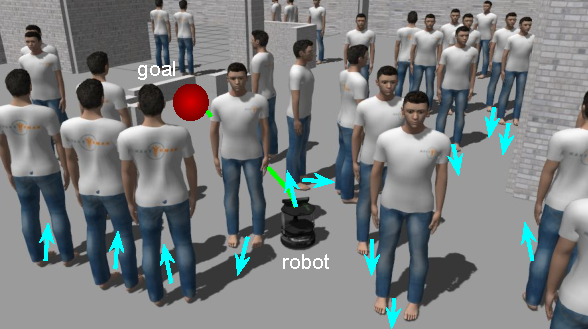
\includegraphics[width=0.77\linewidth]{figures/fig_gazebo_simulation_crowded.pdf}
        \label{fig:gazebo_navigation}
    } 
    %\vspace{0.01cm}
    \subfigure[Real-world outdoor environment]
    {
        \centering
        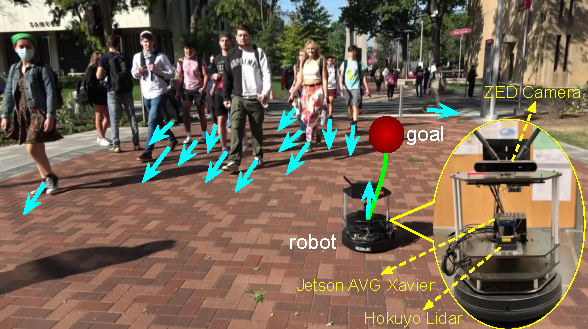
\includegraphics[width=0.77\linewidth]{figures/fig_real_world_outdoor.pdf}
        \label{fig:real_world_navigation}
    }%
     \bcaption[Illustration of the robot navigation problem.]{
    \ul{ Illustration of the robot navigation problem.}
     The robot navigates through crowds in a simulated indoor environment and a real-world outdoor environment. 
     The robot is following a nominal path (green line) to the goal (red disk) while avoiding pedestrians (blue arrows show current velocity).
    }
    \label{fig:navigation_examples}
\end{figure}




